\section{Experiment setup} % (fold)
\label{sec:experiment_setup}

% section experiment_setup (end)
The following diagram is a visualization of the setup and different components we used for our end-to-end latency experiment.\\
\newline

% Please add the following required packages to your document preamble:
% \usepackage{booktabs}


\begin{table}[H]
\centering
\caption{Experiment Components}
\label{tab:experimentComponents}
\renewcommand{\arraystretch}{1.2}
\begin{tabular}{@{}ll@{}}
\toprule
\textbf{ID} & \textbf{Description}            \\ \midrule
\textbf{1}  & USB cable                       \\
\textbf{2}  & Sensor node                     \\
\textbf{3}  & Bluetooth Low Energy Connection \\
\textbf{4}  & Android Gateway Software        \\
\textbf{5}  & WiFi                            \\
\textbf{6}  & Meteor Monitoring server        \\
\textbf{7}  & Time Synchronizer server        \\
\textbf{8}  & Laptop                          \\
\textbf{9}  & Web Client                      \\
\textbf{10} & Ethernet connection             \\ \bottomrule
\end{tabular}
\end{table}

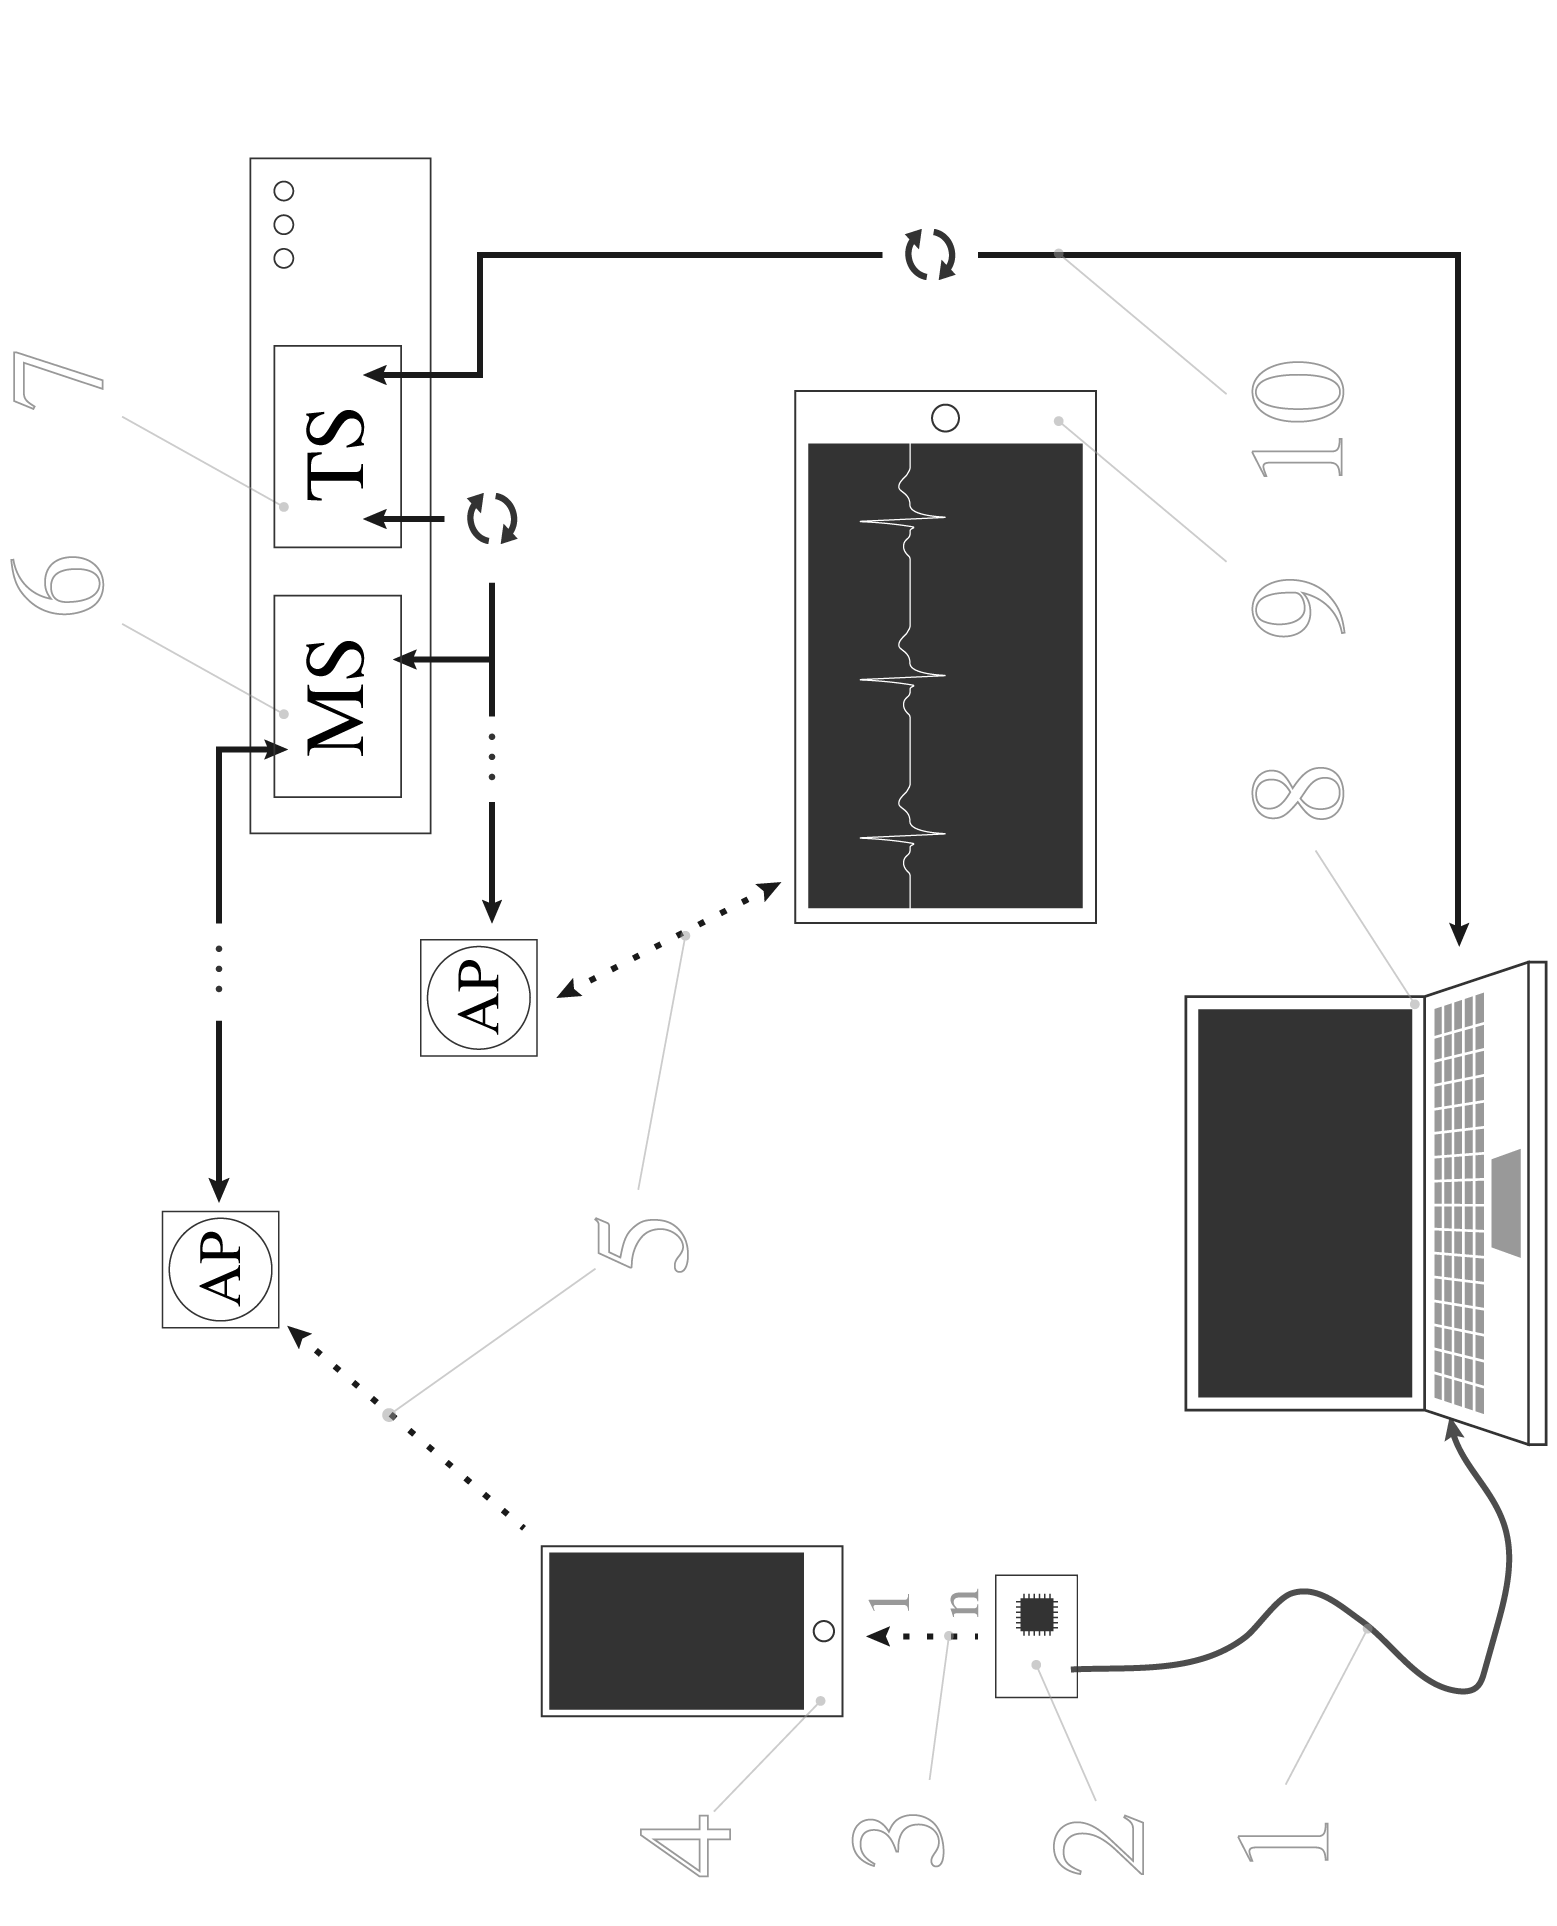
\includegraphics[scale=.25]{img/figures/end-to-end4.png}